%\documentclass[wsdraft]{ws-procs11x85}

\documentclass{ws-procs11x85}
\usepackage{ws-procs-thm}           % comment this line when `amsthm / theorem / ntheorem` package is used

\begin{document}

\title{For proceedings contributors: Using World Scientific's\\ ws-procs11x85 document class with \LaTeX2e\footnote{Type the title of the paper, authors' names with the first letter of important words capitalized.}}

\author{First Author$^\dag$ and Second Author}

\address{University Department, University Name,\\
City, State ZIP/Zone, Country\\
$^\dag$E-mail: ab\_author@university.com\\
www.university\_name.edu}

\author{Third Author}

\address{Group, Laboratory, Street,\\
City, State ZIP/Zone, Country\\
E-mail: an\_author@laboratory.com}

\begin{abstract}
This article explains how to use World Scientific's ws-procs11x85
document class written in \LaTeX2e. This article was typeset using
ws-procs11x85.cls and may be used as a template for your contribution.
\end{abstract}

\keywords{Style file; \LaTeX; Proceedings; World Scientific Publishing.}

% required
\copyrightinfo{\copyright\ 2016 The Authors. Open Access chapter published by World Scientific Publishing Company and distributed under the terms of the Creative Commons Attribution Non-Commercial (CC BY-NC) 4.0 License.}

% required
\bodymatter

\section{Using Other Packages}\label{aba:sec1}
The class file loads the packages {\tt amsfonts, amsmath, amssymb,
chapterbib, cite, dcolumn, rotating} and {\tt url} at
startup. Please try to limit your use of additional packages as they
often introduce incompatibilities. This problem is not specific to
the WSPC styles; it is a general \LaTeX{} problem. Check this
article to see whether the required functionality is already
provided by the WSPC class file. If you do need additional packages,
send them along with the paper. In general, you should use standard
\LaTeX{} commands as much as possible.

\section{Layout}
In order to facilitate our processing of your article, please give
easily identifiable structure to the various parts of the text by
making use of the usual \LaTeX{} commands or by using your own commands
defined in the preamble, rather than by using explicit layout
commands, such as \verb|\hspace, \vspace, \large, \centering|,
etc.~Also, do not redefine the page-layout parameters.

\section{User Defined Macros}
User defined macros should be placed in the preamble of the article,
and not at any other place in the document. Such private
definitions, i.e. definitions made using the commands
\verb|\newcommand,| \verb|\renewcommand,| \verb|\newenvironment| or
\verb|\renewenvironment|, should be used with great care. Sensible,
restricted usage of private definitions is encouraged. Large macro
packages and definitions that are not used in this example article
should be avoided. Please do not change the existing environments,
commands and other standard parts of \LaTeX.

\section{Using WS-procs11x85}
\subsection{Input used to produce this paper}
\begin{verbatim}
\documentclass{ws-procs11x85}
\begin{document}
\title{For proceedings ...}
\author{First Author$^*$ ...}
\address{University ...}
\author{Second Author}
\address{Group, Laboratory, ...}
\begin{abstract}
This article...
\end{abstract}
\keywords{Style file; ...}
\bodymatter
\section{Using Other Packages}
The class file has...
\appendix{About the Appendix}
Appendices should be...
\bibliographystyle{ws-procs11x85}
\bibliography{ws-pro-sample}
\end{document}
\end{verbatim}

\section{Sectional Units}
Sectional units are obtained in the usual way, i.e. with the \LaTeX{}
commands \verb|\section|, \verb|\subsection|,
\verb|\subsubsection| and \verb|\paragraph|.

\section{Section}
This is just an example.

\subsection{Subsection}
This is just an example.

\subsubsection{Subsubsection}
This is just an example.

\paragraph{Paragraph}
This is just an example.

\section*{Unnumbered Section}
Unnumbered sections can be obtained by using \verb|\section*|.

\section{Lists of Items}
Lists are broadly classified into four major categories that can
randomly be used as desired by the author:
\begin{alphlist}[(d)]
\item Numbered list.
\item Lettered list.
\item Unnumbered list.
\item Bulleted list.
\end{alphlist}

\subsection{Numbered and lettered list}

\begin{arabiclist}[(5)]
\item The \verb|\begin{arabiclist}[]| command is used for the arabic
number list (arabic numbers appearing within parenthesis), e.g.,
(1), (2), etc.

\smallskip

\item The \verb|\begin{romanlist}[]| command is used for the roman
number list (roman numbers appearing within parenthesis), e.g., (i),
(ii), etc.

\smallskip

\item The \verb|\begin{Romanlist}[]| command is used for the cap roman
\hbox{number list} (cap roman numbers appearing within parenthesis),
e.g., (I), (II), etc.

\smallskip

\item The \verb|\begin{alphlist}[]| command is used for the alphabetic
list (alphabets appearing within parenthesis),
e.g., (a), (b), etc.

\smallskip

\item The \verb|\begin{Alphlist}[]| command is used for the cap
alphabetic list (cap alphabets appearing within parenthesis),
e.g., (A), (B), etc.
\end{arabiclist}
Note: For all the above mentioned lists (with the exception of
alphabetic list), it is obligatory to enter the last entry's number
in the list within the square bracket, to enable unit alignment.

\subsection{Bulleted and unnumbered list}

The \verb|\begin{itemlist}| command is used for the bulleted list.
The \verb|\begin{unnumlist}| command is used for creating the
  unnumbered list with the turnovers hangindent by 1\,pica.

Lists may be laid out with each item marked by a dot:
\begin{itemlist}
\item item one
\item item two
\item item three
\item item four.
\end{itemlist}

Items may also be numbered with lowercase Roman numerals:
\begin{romanlist}[(iv)]
\item item one
\item item two
    \begin{alphlist}[(a)]
    \item lists within lists can be numbered with lowercase alphabets
    \item second item.
    \end{alphlist}
\item item three.
\end{romanlist}

\section{Theorems and Definitions}

The following environments are available by default
with WSPC document styles:

\begin{center}
{\tablefont
\begin{tabular}{ll}
\toprule
Environment & Heading\\\colrule
\verb|algorithm| & Algorithm\\
\verb|answer| & Answer\\
\verb|assertion| & Assertion\\
\verb|assumption| & Assumption\\
\verb|case| & Case\\
\verb|claim| & Claim\\
\verb|comment| & Comment\\
\verb|condition| & Condition\\
\verb|conjecture| & Conjecture\\
\verb|convention| & Convention\\
\verb|corollary| & Corollary\\
\verb|criterion| & Criterion\\
\verb|definition| & Definition\\
\verb|example| & Example\\
\verb|lemma| & Lemma\\
\verb|notation| & Notation\\
\verb|note| & Note\\
\verb|observation| & Observation\\
\verb|problem| & Problem\\
\verb|proposition| & Proposition\\
\verb|question| & Question\\
\verb|remark| & Remark\\
\verb|solution| & Solution\\
\verb|step| & Step\\
\verb|summary| & Summary\\
\verb|theorem| & Theorem \\\botrule
\end{tabular}}\label{aba:theo}
\end{center}

\noindent{\bf Input:}

\begin{verbatim}
\begin{theorem}
We have $\# H^2 (M \supset N) < ...
\label{aba:the1}
\end{theorem}
\end{verbatim}

\noindent{\bf Output:}

\begin{theorem}
We have $\# H^2 (M \supset N) < \infty$ for an inclusion $M \supset N$ of
factors of finite index.
\label{aba:the1}
\end{theorem}

\noindent{\bf Input:}

\begin{verbatim}
\begin{theorem}[Longo, 1998]
For a given $Q$-system ...
\[ N = \{x \in N; ... \}\,, \]
and $E_\Xi (\cdot) = T^* ...\label{aba:the2}
\end{theorem}
\end{verbatim}

\noindent{\bf Output:}

\begin{theorem}[Longo, 1998]
For a given $Q$-system...
\[
N = \{x \in N; T x = \gamma (x) T, T x^* = \gamma (x^*) T\}\,,
\]
and $E_\Xi (\cdot) = T^* \gamma (\cdot) T$ gives a conditional
expectation onto $N$.
\label{aba:the2}
\end{theorem}

\LaTeX{} provides \verb|\newtheorem| to create new theorem
environments. To add theorem-type environments to an article, use

\begin{verbatim}
\newtheorem{example}{Example}[section]
\let\Examplefont\upshape
\def\Exampleheadfont{\bfseries}
\begin{example}
We have $\# H^2 (M \supset N) < ...
\end{example}
\end{verbatim}

For details see the \LaTeX{} user manual.\cite{lamp94,ams04}

\subsection{Proofs}
The WSPC document styles also provide a predefined proof environment for proofs.
The proof \hbox{environment} produces the heading
`Proof' with appropriate spacing and punctuation. It also appends a `Q.E.D.' symbol, $\square$, at the end of a proof, e.g.

\begin{verbatim}
\begin{proof}
This is just an example.
\end{proof}
\end{verbatim}

\noindent to produce

\begin{proof}
This is just an example.
\end{proof}

The proof environment takes an argument in curly
braces, which allows you to substitute a different name for the standard
`Proof'. If you want to display, `Proof of Lemma', then write e.g.

\begin{verbatim}
\begin{proof}[Proof of Lemma]
This is just an example.
\end{proof}\end{verbatim}

\noindent produces

\begin{proof}[Proof of Lemma]
This is just an example.
\end{proof}

\section{Programs and Algorithms}
Fragments of computer programs and descriptions of algorithms should be
prepared as if they were normal text. Use the same fonts for keywords,
variables, etc., as in the text; do not use small typeface sizes to make program
fragments and algorithms fit within the margins set by the document style.
An example with only the tabbing environment and one new definition:
\begin{verbatim}
\newcommand{\keyw}[1]{{\bf #1}}
\begin{tabbing}
\quad \=\quad \=\quad \kill
\keyw{for} each $x$ \keyw{do} \\
\> \keyw{if} extension$(p, x)$ \\
\> \> \keyw{then} $E:=E\cup\{x\}$\\
\keyw{return} $E$
\end{tabbing}
\end{verbatim}

\newcommand{\keyw}[1]{{\bf #1}}
{\small{
\begin{tabbing}
\quad \=\quad \=\quad \kill
\keyw{for} each $x$ \keyw{do} \\
\> \keyw{if} extension$(p, x)$ \\
\> \> \keyw{then} $E:=E\cup\{x\}$\\
\keyw{return} $E$
\end{tabbing}
}}

\section{Mathematical Formulas}
\paragraph{Inline:}
For in-line formulas use \verb|\( ... \)| or \verb|$ ... $|. Avoid
built-up constructions, for example fractions and matrices, in
in-line formulas. Fractions in inline can be typed with a solidus, e.g. \verb|x+y/z=0|.

\paragraph{Display:}
For numbered display formulas, use the displaymath
environment:

\verb|\begin{equation}...\end{equation}|.

And for unnumbered display formulas, use
\verb|\[ ... \]|. For numbered displayed,
one-line formulas always use the equation environment. Do not use
\verb|$$ ... $$|.

For example, the input for:
\begin{equation}
\mu(n, t) = \frac{\sum\limits^\infty_{i=1}1
(d_i < t, N(d_i) = n)}
{\int\limits^t_{\sigma=0}1(N(\sigma)=n)d\sigma}.\label{aba:eq1}
\end{equation}

\noindent is:

\begin{verbatim}
\begin{equation}
\mu(n, t) = \frac{\sum ...}{\int ...}.
\label{aba:eq1}
\end{equation}
\end{verbatim}

For displayed multi-line formulas, use the \verb|eqnarray| environment. For example,

\begin{verbatim}
\begin{eqnarray}
\zeta\mapsto\hat{\zeta}& =
   &a\zeta+b\eta\label{aba:appeq2}\\
\eta\mapsto\hat{\eta}& =
   &c\zeta+d\eta\label{aba:appeq3}
\end{eqnarray}
\end{verbatim}

\noindent produces:
\begin{eqnarray}
\zeta\mapsto\hat{\zeta}& =
        &a\zeta+b\eta\label{aba:appeq2}\\
\eta\mapsto\hat{\eta}& =
        &c\zeta+d\eta\label{aba:appeq3}
\end{eqnarray}

\LaTeX\ does not break long equations to make them fit within the
margins as it does with normal text. It is therefore up to you to
format the equation appropriately (if they overrun the margin.) This
typically requires some creative use of an eqnarray to get elements
shifted to a new line and to align nicely, e.g.,
\begin{eqnarray}
\left(1+x\right)^n &=& 1 + nx + \frac{n\left(n-1\right)}{2!}x^2 \nonumber\\
  & & + \frac{n\left(n-1\right)\left(n-2\right)}{3!}x^3 \nonumber\\
  & & + \frac{n\left(n-1\right)\left(n-2\right)\left(n-3\right)}{4!}x^4 \nonumber\\
  & & + \ldots n{\rm th}.
\end{eqnarray}

Superscripts and subscripts that are words or abbreviations, as in
\( \sigma_{\mathrm{low}} \), should be typed as roman letters;
this is done as \verb|\( \sigma_{\mathrm{low}} \)|
instead of \( \sigma_{low} \) done with \verb|\( \sigma_{low} \)|.

For geometric functions, e.g.~exp, sin, cos, tan, etc., please use the macros
\verb|\sin, \cos, \tan|. These macros give proper spacing in mathematical formulas.

It is also possible to use the \AmS-\LaTeX{}
package,\cite{ams04} which can be obtained from the \AmS\ and various \TeX{}
archives.

\section{Floats}
\subsection{Tables}
Put tables and figures in text using the table and figure environments,
and position them near the first reference of the table or figure in
the text. Please avoid long captions in figures and tables.

\paragraph{Input:}

\begin{verbatim}
\begin{table}[h]
\tbl{... table caption ...}
{\begin{tabular}{@{}lcccr@{}}\toprule
ID & $m$ & $R^2$ & $x_2$ & Times\\ \colrule
11 & 100 & 3135 & 1138 & $<98$ sec\\
11 & 100 & 3135 & 1138 & $<98$ sec\\
12 & 100 & 3135 & 1138 & $<99$ sec\\
13 & 100 & 3135 & 1138 & $<100$ sec\\
14 & 100 & 3135 & 1138 & $<101$ sec\\
15 & 100 & 3135 & 1138 & $<102$ sec\\ \botrule
\end{tabular}}\label{aba:tbl1}
\end{table}
\end{verbatim}

\noindent {\bf Output:}

\begin{table}[h]
\tbl{... table caption ...}
{\begin{tabular}{@{}lcccr@{}}
\toprule
ID & $m$ & $R^2$ & $x_2$ & Times\\ \colrule
11 & 100 & 3135 & 1138 & $<98$ sec\\
12 & 100 & 3135 & 1138 & $<99$ sec\\
13 & 100 & 3135 & 1138 & $<100$ sec\\
14 & 100 & 3135 & 1138 & $<101$ sec\\
15 & 100 & 3135 & 1138 & $<102$ sec\\ \botrule
\end{tabular}}\label{aba:tbl1}
\end{table}

By using \verb|\tbl| command in table environment, long captions will be justified to the table width while the short or single line captions are centered.
\begin{verbatim}
\begin{table}[h]
\tbl{table caption}
{tabular environment}
\label{tblabel}
\end{table}
\end{verbatim}
For most tables, the horizontal rules are obtained by:

\noindent
\begin{tabular}{ll}
{\bf toprule} & one rule at the top\\
{\bf colrule}& one rule separating column\\ & heads from data cells\\
{\bf botrule}& one bottom rule\\
{\bf Hline} & one thick rule at the top and\\ & bottom of the tables with\\ & multiple column heads\\
\end{tabular}

To avoid the rules sticking out at either end
of the table, add \verb|@{}| before the first and after the last descriptors, e.g.
{@{}llll@{}}. Please avoid vertical rules in tables.
But if you think the vertical rule is a must,
you can use the standard \LaTeX{} \verb|tabular| environment.

Headings which span for more than one column should be set using
\verb|\multicolumn{#1}{#2}{#3}| where \verb|#1| is the number of
columns to be spanned, \verb|#2| is the argument for the alignment
of the column head which may be either {c} --- for center
alignment; {l} --- for left alignment; or {r} --- for right
alignment, as desired by the users. Use {c} for column heads as
this is the WS style and \verb|#3| is the heading.

For the footnotes in the table environment the command is
\verb|\begin{tabnote}<text>\end{tabnote}|.

Tables should have a uniform style throughout the
proceedings volume. It does not matter how you place the
inner lines of the table, but we would prefer the border lines to be
of the style as shown in our sample tables.
For the inner lines of the table, it looks better
if they are kept to a minimum.

\subsection{Figures}
\noindent A figure is obtained with the following commands

\begin{verbatim}
\begin{figure}[h]
\centerline{
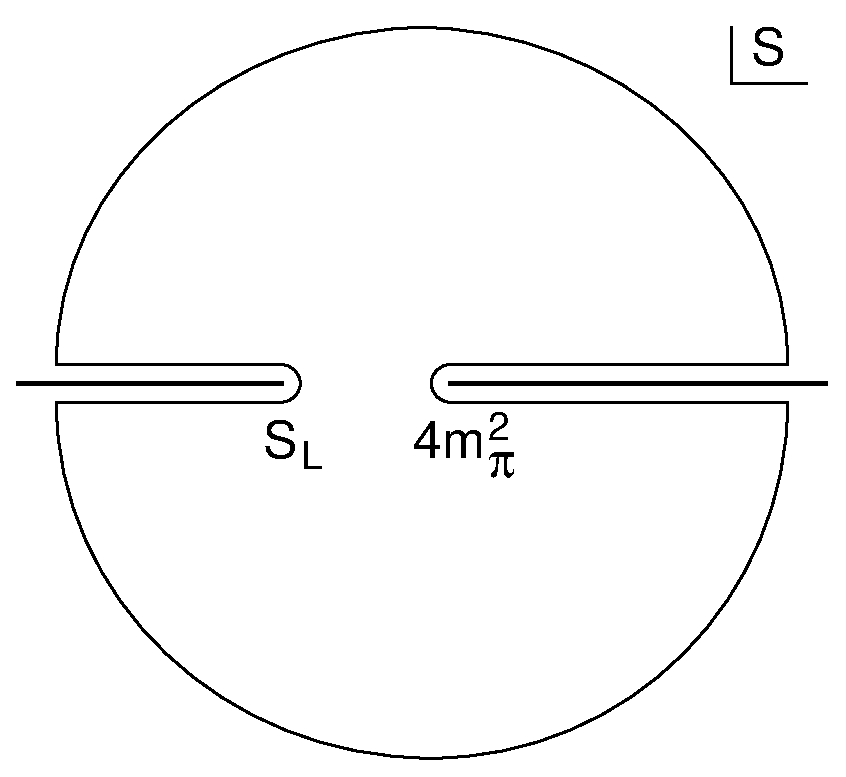
\includegraphics[width=4.5cm]{procs-fig1}
}
\caption{...caption here...}
\label{aba:fig1}
\end{figure}
\end{verbatim}

\begin{figure}[h]
\centerline{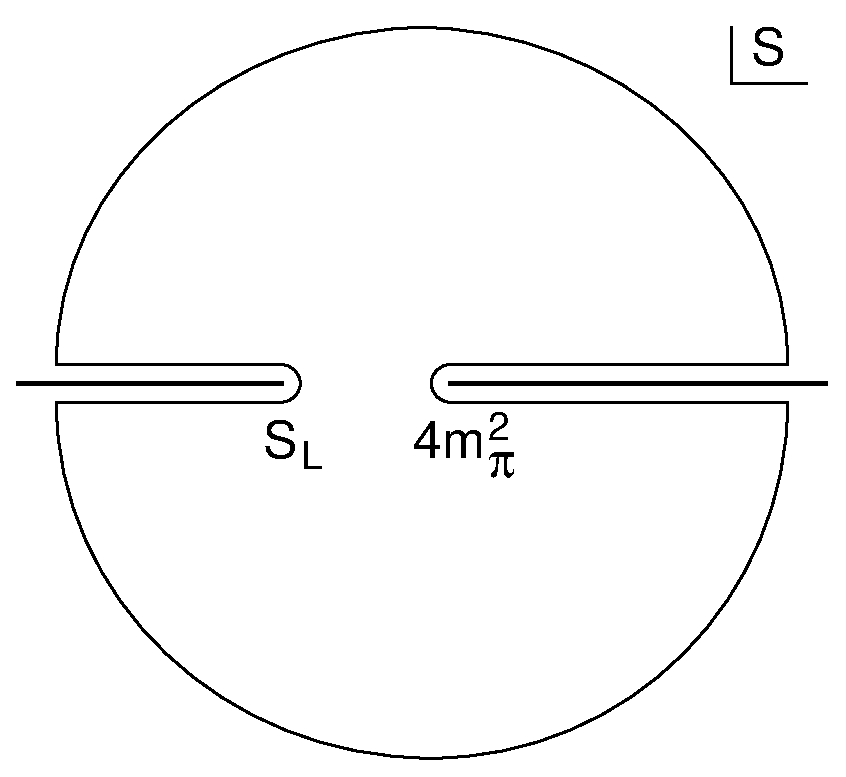
\includegraphics[width=4.5cm]{procs-fig1}}
\caption{ ... caption here ... }
\label{aba:fig1}
\end{figure}

The preferred graphics formats are TIF and Encapsulated
PostScript (EPS) for any type of image. Our
\TeX\ installation requires EPS, but we can easily convert TIF to EPS.
Many other formats, e.g. PICT (Macintosh), WMF (Windows) and various proprietary
formats, are not suitable. Even if we can read such files, there is no guarantee
that they will look the same on our systems as on yours.

Adjust the scaling of the figure until it is correctly positioned,
and remove the declarations of the lines and any anomalous spacing.

\begin{sidewaysfigure}
\begin{center}
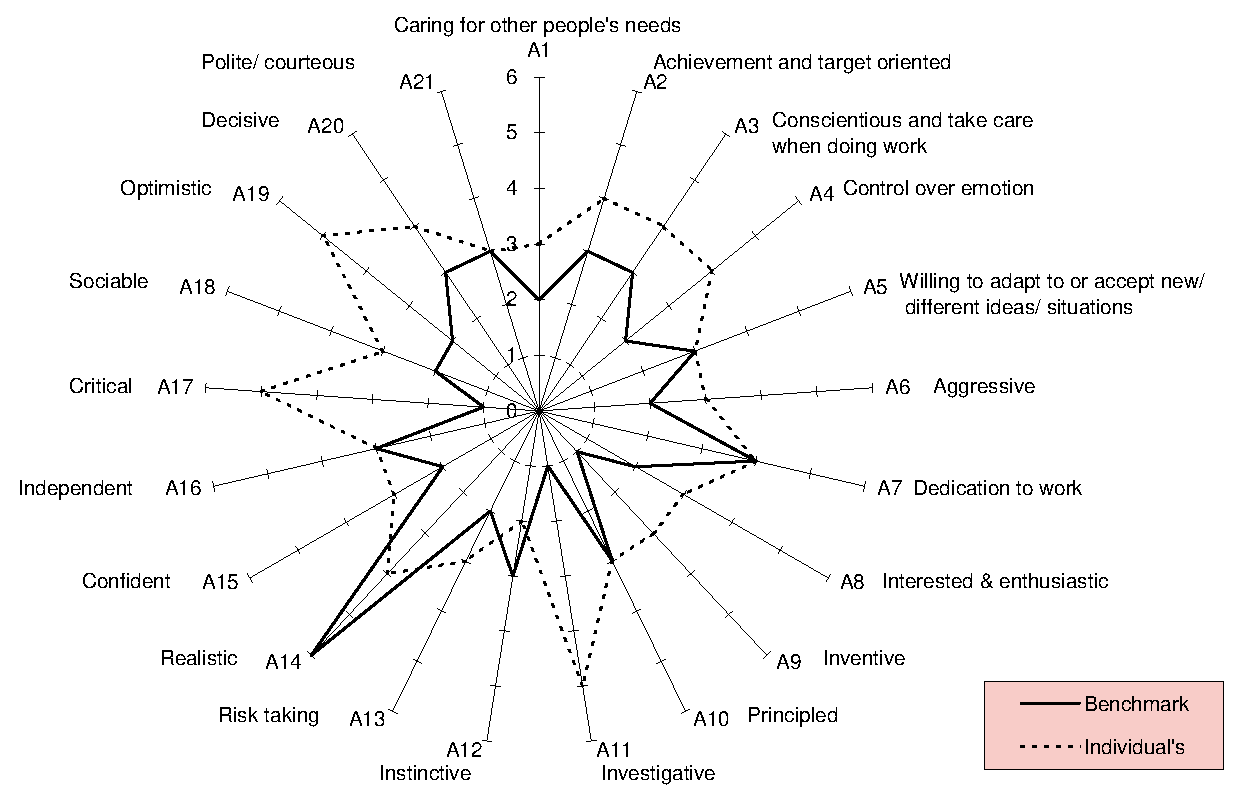
\includegraphics[width=6in]{procs-fig2}
\end{center}
\caption{The bifurcating response curves of system
$\alpha=0.5$, $\beta=1.8$; $\delta=0.2$, $\gamma=0$: (a)
$\mu=-1.3$; and\break (b) $\mu=0.3$.}
\label{aba:fig2}
\end{sidewaysfigure}

\def\p{\phantom{$-$}}
\def\pc{\phantom{,}}
\def\p0{\phantom{0}}
\begin{sidewaystable}
\tbl{Positive values of $X_0$ by eliminating $Q_0$ from
Eqs.~(15) and (16) for different values of the parameters $f_0$,
$\lambda_0$ and $\alpha_0$ in various dimension.}
{\begin{tabular}{@{}ccccccccccc@{}}
\toprule\\[-6pt]
$f_0$ &$\lambda_0$ &$\alpha_0$
&\multicolumn{8}{c}{Positive roots ($X_0$)}\\[3pt]
\hline\\[-6pt]
&& &4D &5D &6D &7D &8D &10D &12D &16D\\[3.5pt]
\hline\\[-6pt]
\phantom{1}$-0.033$ &0.034 &\phantom{0}0.1\phantom{.01}
&6.75507,\p0 &4.32936,\p0 &3.15991,\p0 &2.44524,\p0
&1.92883,\p0 &0.669541, &--- &---\\[3.5pt]
&&&1.14476\pc\p0 &1.16321\pc\p0 &1.1879\pc\phantom{00}
&1.22434\pc\p0 &1.29065\pc\p0
&0.415056\pc\\[3.5pt]
\phantom{1}$-0.1$\phantom{33} &0.333 &\phantom{0}0.2\phantom{.01}
&3.15662,\p0 &1.72737,\p0 &--- &--- &--- &--- &--- &---\\[3.5pt]
&&&1.24003\pc\p0 &1.48602\pc\p0\\[3.5pt]
\phantom{1}$-0.301$ &0.302 &0.001
&2.07773,\p0 &--- &--- &--- &--- &--- &--- &---\\[3.5pt]
&&&1.65625\pc\p0\\[3.5pt]
\phantom{1}$-0.5$\phantom{01} &0.51\phantom{2} &\phantom{0}0.001
&--- &--- &--- &--- &--- &--- &--- &---\\[3.5pt]
$\phantom{1-}$0.1\phantom{01} &0.1\phantom{02}
&\phantom{0}2\phantom{.001} &1.667,\phantom{000} &1.1946\phantom{00,}
&--- &--- &--- &--- &--- &---\\[3.5pt]
&&&0.806578\pc &0.858211\pc\\[3.5pt]
$\phantom{1-}$0.1\phantom{01} &0.1\phantom{33} &10\phantom{.001}
&0.463679\pc &0.465426\pc &0.466489\pc &0.466499\pc
&0.464947\pc &0.45438\pc\p0 &0.429651\pc &0.35278\pc\\[3.5pt]
$\phantom{1-}$0.1\phantom{01} &1\phantom{.333}
&\phantom{0}0.2\phantom{01}
&--- &--- &--- &--- &--- &--- &--- &---\\[3.5pt]
$\phantom{1-}$0.1\phantom{01} &5\phantom{.333}
&\phantom{0}5\phantom{.001}
&--- &--- &--- &--- &--- &--- &--- &---\\[3.5pt]
$\phantom{-0}$1\phantom{.033} &0.001 &\phantom{0}2\phantom{.001}
&0.996033, &0.968869, &0.91379,\p0 &0.848544,&0.783787, &0.669541,
&0.577489, &---\\[3.5pt]
&&&0.414324\pc &0.41436\pc\p0 &0.414412\pc &0.414489\pc &0.414605\pc
&0.415056\pc &0.416214\pc\\[3.5pt]
\phantom{10}\phantom{.033} &0.001 &\phantom{0}0.2\phantom{01}
&0.316014, &0.309739, &--- &--- &--- &--- &--- &---\\[3.5pt]
&&&0.275327\pc &0.275856\pc\\[3.5pt]
\phantom{10}\phantom{.033} &0.1\phantom{33}
&\phantom{0}5\phantom{.001}
&0.089435\pc &0.089441\pc &0.089435\pc &0.089409\pc &0.08935\pc\p0
&0.089061\pc &0.088347\pc &0.084352\pc\\[3.5pt]
\phantom{10}\phantom{.033} &1\phantom{.333} &\phantom{0}3\phantom{.001}
&0.128192\pc &0.128966\pc &0.19718,\p0 &0.169063, &0.142103,
&--- &--- &---\\[3.5pt]
&&&& &0.41436\pc\p0 &0.414412\pc &0.414489\pc\\[3pt]
\Hline
\end{tabular}}
\label{aba:tbl3}
\end{sidewaystable}

Very large figures and tables should be placed on a separate page
by themselves. Landscape tables and figures can be typeset with the following environments:
\begin{itemize}
\item \verb|sidewaystable| and
\item \verb|sidewaysfigure|.
\end{itemize}

\noindent {\bf Example:}

\begin{verbatim}
\begin{sidewaysfigure}
\begin{center}
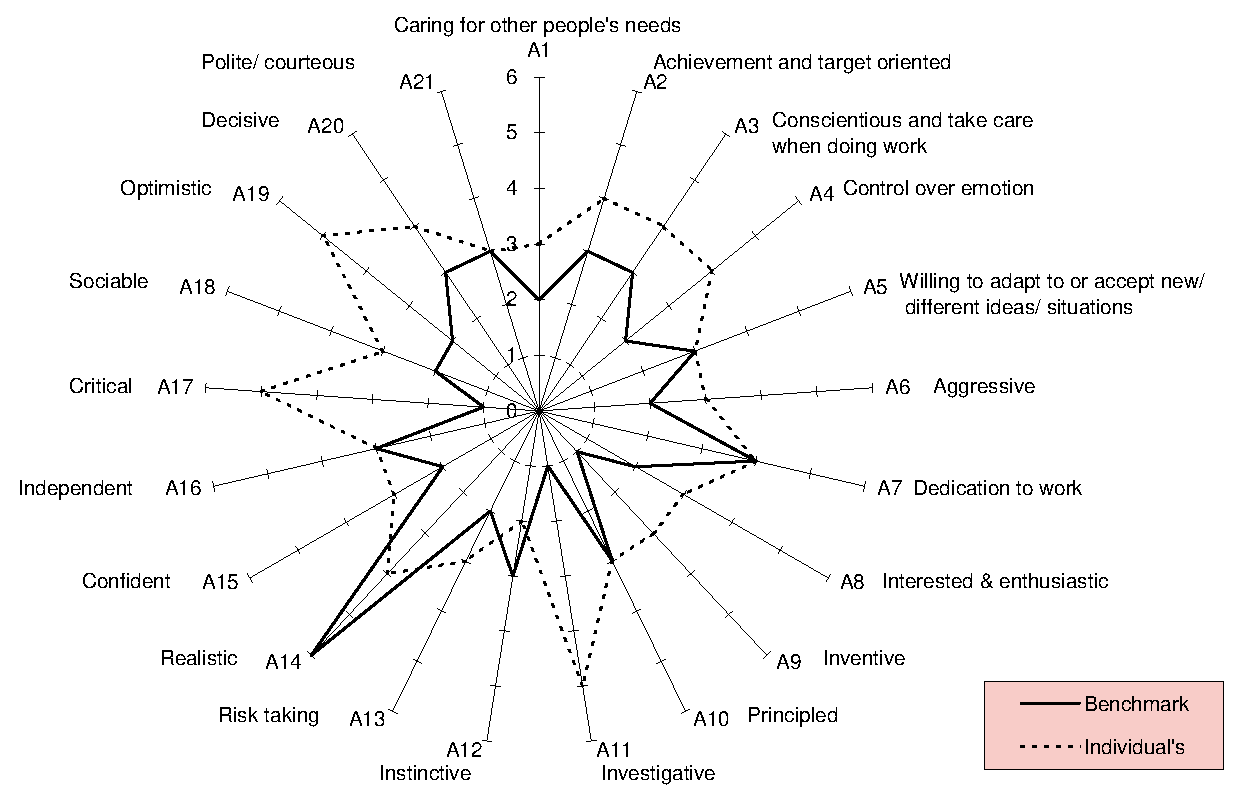
\includegraphics[width=6in]{procs-fig2}
\end{center}
\caption{Caption ...}
\label{aba:fig2}
\end{sidewaysfigure}
\end{verbatim}

\begin{verbatim}
\begin{sidewaystable}
\tbl{Positive values of ...}
{\begin{tabular}{@{}ccccccccccc@{}}
...
\end{tabular}}
\label{aba:tbl3}
\end{sidewaystable}
\end{verbatim}

\section{Cross-references}
Use \verb|\label| and \verb|\ref| for cross-references to
equations, figures, tables, sections, subsections, etc., instead
of plain numbers. Every numbered part to which one wants to refer,
should be labeled with the instruction \verb|\label|.
For example:
\begin{verbatim}
\begin{equation}
\mu(n, t) = \frac{\sum ...}{\int ...}.
\label{aba:eq1}
\end{equation}
\end{verbatim}
With the instruction \verb|\ref| one can refer to a numbered part
that has been labeled:
\begin{verbatim}
..., see also Eq. (\ref{aba:eq1})
\end{verbatim}

The \verb|\label| instruction should be typed
\begin{itemize}
\item immediately after (or one line below), but not inside the argument of
a number-generating instruction such as \verb|\section| or \verb|\caption|, e.g.: \verb|\caption{Caption}\label{aba:fig1}|.
\item roughly in the position where the number appears, in environments
such as an equation,
\item labels should be unique, e.g., equation 1 can be labeled as
\verb|\label{aba:eq1}|, where `{\tt aba}' is author's initial and
`{\tt eq1}' the equation number.
\end{itemize}

\section{Citations}
We have used \verb|\bibitem| to produce the bibliography. Citations in the
text use the labels defined in the bibitem declaration, e.g.,
the first paper by Jarlskog\cite{jarl88} is cited using the command
\verb|\cite{jarl88}|. Bibitem labels should be unique.

For multiple citations, do not use \verb|\cite{1}|, \verb|\cite{2}|, but use
\verb|\cite{1,2}| instead.

When the reference forms part of the sentence, it should not
be typed in superscripts, e.g.: ``One can show from
Ref.~\refcite{jarl88} that $\ldots$'', ``See
Refs.~\refcite{lamp94} and \refcite{ams04} for more details.''
This is done using the \LaTeX{} command: ``\verb|Ref.~\refcite{name}|''.

\section{Footnotes}
Footnotes are denoted by a Roman letter superscript in the text. Footnotes can be used as

\paragraph{Input:}

\begin{verbatim}
... total.\footnote{Sample footnote.}
\end{verbatim}

\paragraph{Output:}

\noindent ... in total.\footnote{Sample footnote text.}

\section{Acknowledgments and Appendices}
Acknowledgments to funding bodies etc.~may be placed in a separate
section at the end of the text, before the Appendices. This should not
be numbered, so use \verb|\section*{Acknowledgments}|.

It is preferable to have no appendices in a short article, but if
it is necessary, then simply use as

\begin{verbatim}
\appendix{About the Appendix}
Appendices should be...
\begin{equation}
\mu(n, t) = ...
\label{app:a1}
\end{equation}
\subappendix{Appendix Sectional Units}
Sectional units are...
\end{verbatim}

\section{References}
References are to be listed in the order cited in the text in Arabic
numerals. \btex\ users, please use our bibliography style file
\verb|ws-procs11x85.bst| for references. Non \btex\ users can list
down their references in the following pattern.

\begin{verbatim}
\begin{thebibliography}{9}

\bibitem{jarl88} C. Jarlskog, in {\it CP Violation} (World Scientific,
   Singapore, 1988).

\bibitem{lamp94} L. Lamport, {\it \LaTeX, A Document Preparation System},
   2nd edition (Addison-Wesley, Reading, Massachusetts, 1994).

\bibitem{ams04} \AmS-\LaTeX{} Version 2 User's Guide (American Mathematical
   Society, Providence, 2004).

\bibitem{best03} B.~W. Bestbury, {\em J. Phys. A} {\bf 36}, 1947 (2003).

\end{thebibliography}
\end{verbatim}

\section{{\btex}ing}

If you use the \btex\ program to maintain your bibliography, you do
not use the \verb|thebibliography| environment. Instead, you should
include
\begin{verbatim}
\bibliographystyle{ws-procs11x85}
\bibliography{ws-pro-sample}
\end{verbatim}

\noindent where \verb|ws-procs11x85| refers to a file \verb|ws-procs11x85.bst|,
which defines how your references will look.
The argument to \verb|\bibliography| refers to the file
\verb|ws-pro-sample.bib|, which should contain your database in
\btex\ format. Only the entries referred to via \verb|\cite| will be
listed in the bibliography.

Sample output using \verb|ws-procs11x85| bibliography style file:

\begin{center}
\tablefont
\begin{tabular}{@{}ll@{}}\toprule
\multicolumn{1}{c}{\btex}\\
\multicolumn{1}{c}{database}  & \multicolumn{1}{c}{Sample citation}\\
\multicolumn{1}{c}{entry type}\\\colrule

article & ... text.\cite{best03,pier02,jame02}\\

proceedings & ... text.\cite{weis94}\\

inproceedings & ... text.\cite{gupt97}\\

book & ... text.\cite{jarl88,rich60}\\

edition & ... text.\cite{chur90}\\

editor & ... text.\cite{benh93}\\

series & ... text.\cite{bake72}\\

tech report & See Refs.~\refcite{hobb92} and \refcite{bria84} for more details\\

unpublished & ... text.\cite{hear94}\\

phd thesis & ... text.\cite{brow88}\\

masters thesis & ... text.\cite{lodh74}\\

incollection & ... text.\cite{dani73}\\

misc & ... text.\cite{davi93}\\
\botrule
\end{tabular}
\end{center}

\appendix{About the Appendix}
Appendices should be used only when absolutely necessary. They
should come before the References.

\begin{table}[b]
\tbl{Macros available for use.}
{\begin{tabular}{@{}ll@{}}\toprule
Macro name&Purpose\\
\colrule
{\tt$\backslash$title}\{{\tt\#1}\} & Article Title\\
{\tt$\backslash$author}\{{\tt\#1}\} & List of all Authors\\
{\tt$\backslash$address}\{{\tt\#1}\} & Address of Author\\
{\tt$\backslash$maketitle} & Formats title page\\
{\tt$\backslash$begin}\{{\tt{abstract}}\} & Start Abstract\\
{\tt$\backslash$end}\{{\tt{abstract}}\} & End Abstract\\
{\tt$\backslash$keywords}\{{\tt\#1}\} & Keywords\\
{\tt$\backslash$bodymatter} & Start body text\\
{\tt$\backslash$section}\{{\tt\#1}\} & Section heading\\
{\tt$\backslash$subsection}\{{\tt\#1}\} & Subsection heading\\
{\tt$\backslash$subsubsection}\{{\tt\#1}\} & Subsubsection heading\\
{\tt$\backslash$section*}\{{\tt\#1}\} & Unnumbered Section head\\
{\tt$\backslash$begin}\{{\tt{itemlist}}\} & Start unnumbered lists\\
{\tt$\backslash$end}\{{\tt{itemlist}}\} & End unnumbered lists\\
{\tt$\backslash$begin}\{{\tt{romanlist}}\} & Start roman lists\\
{\tt$\backslash$end}\{{\tt{romanlist}}\} & End roman lists\\
{\tt$\backslash$begin}\{{\tt{alphlist}}\} & Start alpha lists\\
{\tt$\backslash$end}\{{\tt{alphlist}}\} & End alpha lists\\
{\tt$\backslash$begin}\{{\tt{proof}}\} & Start of Proof\\
{\tt$\backslash$end}\{{\tt{proof}}\} & End of Proof\\
{\tt$\backslash$begin}\{{\tt{theorem}}\} & Start of Theorem\\
{\tt$\backslash$end}\{{\tt{theorem}}\} & End of Theorem\\&\quad See Page \pageref{aba:theo} for detailed list\\
{\tt$\backslash$appendix}\{{\tt\#1}\} & Appendix heading\\
{\tt$\backslash$begin}\{{\tt{thebibliography}}\} & Start of numbered reference list\\
{\tt$\backslash$end}\{{\tt{thebibliography}}\} & End of numbered reference list\\[6pt]
\multicolumn{2}{@{}l}{Macros available for Table/Figures}\\[3pt]
{\tt figure} & Single column figures\\
{\tt sidewaysfigure} & landscape figures\\
{\tt table} & Single column tables\\
{\tt sidewaystable} & landscape tables\\[3pt]
\multicolumn{2}{@{}l}{Horizontal rules for tables}\\
{\tt$\backslash$toprule} & one rule at the top\\
{\tt$\backslash$colrule} & one rule separating column heads from\\ & data cells\\
{\tt$\backslash$botrule} & one bottom rule\\
{\tt$\backslash$Hline} & one thick rule at the top and bottom of\\ & the tables with multiple column heads\\
\botrule
\end{tabular}}
\end{table}

Unnumbered appendix sections can be obtained using \verb|\section*|.

\noindent\begin{eqnarray}
\zeta\mapsto\hat{\zeta}&=&a\zeta+b\eta\label{aba:app1}\\
\eta\mapsto\hat{\eta}&=&c\zeta+d\eta\label{aba:app2}
\end{eqnarray}

Number displayed equations
occurring in the appendix in this way, e.g.~(\ref{aba:app1}), (\ref{aba:app2}),
etc.

The numbered citations can appear in two ways:

\begin{arabiclist}
\item Superscript$^1$  (default)
      \verb| - \usepackage{ws-procs11x85}|

\item Bracketed [1]
      \verb|        - \usepackage[square]{ws-procs11x85}|
\end{arabiclist}

The contributors are advised to consult the proceedings editor before choosing the citation style \verb|square|.

\bibliographystyle{ws-procs11x85}
\bibliography{ws-pro-sample}

\end{document}